
\documentclass[conference]{IEEEtran}
\IEEEoverridecommandlockouts
% The preceding line is only needed to identify funding in the first footnote. If that is unneeded, please comment it out.
\usepackage{cite}
\usepackage{amsmath,amssymb,amsfonts}
\usepackage{algorithmic}
\usepackage{graphicx}
\usepackage{textcomp}
\usepackage{xcolor}
\usepackage{tikz}
\usetikzlibrary{positioning,fit,arrows.meta,shapes.geometric,calc}


\def\BibTeX{{\rm B\kern-.05em{\sc i\kern-.025em b}\kern-.08em
    T\kern-.1667em\lower.7ex\hbox{E}\kern-.125emX}}
\begin{document}

\title{A model for object detection and semantic segmentation applicable to the CamVid dataset\\
{\footnotesize \textsuperscript{*}Based on YoloV3 and Deeplabv3 architectures - COMP0248}
}

\author{\IEEEauthorblockN{Jiaqi Yao}}

\maketitle

\begin{abstract}


\end{abstract}

\begin{IEEEkeywords}
object detection, semantic segmentation, YoloV3, Deeplabv3, CamVid dataset
\end{IEEEkeywords}

\section{Introduction}
% 计算机视觉在近年来取得了显著的进展,然而机器仍然难以像人类一样准确理解城市环境。因此,在本课程作业中,我们尝试使机器能够准确识别和分割街景中的对象,使用CamVid(Cambridge-driving Video)数据集。

% 具体来说,这涉及到机器具有识别道路、建筑物、行人、车辆和其他元素的能力,就像人类通过步行或驾驶在城市中导航一样。

% 此外,传统的计算机视觉模型通常由于数据不平衡而面临困难,例如公交车等某些类别。此外,由于CamVid数据集中类别较少(与COCO相比),我们无法使用大多数复杂的CNN和目标检测模型进行迁移学习和微调。

% 在本文中,我们仅关注CamVid数据集中的五个常见类别,即汽车、行人、自行车、摩托车和公共汽车。因此,类别不平衡的问题将是数据集中的一个非常突出的特征,我们必须针对类别不平衡的问题。

% 为了解决这些挑战,我们将根据YoloV3和Deeplabv3架构的思想重新编程和构建模型,分别是目标检测和语义分割。为了防止过拟合,我们将简化和修改大部分架构,以便我们可以在小数据集(如CamVid数据集)上训练模型,并评估其在mAP、IoU和其他指标方面的性能。我们还将探索各种处理类别不平衡的技术,并分析它们对模型性能的影响。
Computer vision has made significant progress in recent years; however, machines still struggle to comprehend urban environments with the same level of understanding as humans. So, in this coursework, we try to enable machines to accurately identify and segment objects in street scenes using the CamVid (Cambridge-driving Video) dataset.
 
Specifily, this involves the robots with the ability to recognize roads, buildings, pedestrians, vehicles, and other elements in their surroundings—like a human navigating a city by walking or driving.

Additionally, traditional computer vision models often face difficulties due to imbalanced data—certain classes, such as buses. Also, due to the lack of classes in CamVid datasets (Compare with COCO), we cannot use most of the complicated CNN and Object detection models with transfer learning and fine-tune.

In this paper, we focus on only five common categories in the camvid dataset, which are cars, pedestrians, bicycles, motorcycles, and buses. So the problem of category imbalance will be a very prominent feature in the dataset, and we have to target the problem of category imbalance.

To address these challenges, we reprogram and build the model with the help of ideas from the YoloV3 and Deeplabv3 architectures, object detection and semantic segmentation, respectively. To prevent overfitting compared to the original model, we will streamline and modify most of the architectures so that we can train the model on small datasets such as the CamVid dataset and evaluate its performance in terms of mAP, IoU, and other metrics. We will also explore various techniques for dealing with class imbalance and analyze their impact on model performance.
\section{Dataset}
% 5 class distribution, preprocessing steps, data visualization etc.
\subsection{CamVid Dataset Overview}
% CamVid 数据集是相比其他数据集(如COCO,Cityscapes))是较小的数据集。其中包含了街景图像和对应的像素级标注,可用于语义分割任务。数据集中包含32个类别,但我们只关注其中的5个类别:汽车、行人、自行车、摩托车和公共汽车并将其他设为背景。 此外,我们还根据对应的像素级标注,生成对应的适用于目标检测的框标注,以便进行目标检测任务。
The CamVid dataset is a relatively small dataset compared to others like COCO and Cityscapes. It consists of street scene images and corresponding pixel-level annotations for semantic segmentation tasks. The dataset contains 32 classes, but we focus only on five classes: cars, pedestrians, bicycles, motorcycles, and buses, with the rest labeled as background. Additionally, we generate bounding box annotations suitable for object detection tasks based on the corresponding pixel-level annotations.

\subsection{Data Preprocessing}
%  对于数据的预处理, camvid提供的标签是灰度的掩码图像,是可以直接被用于语义分割的训练。 我们需要做的就是增加一个过滤器,将原有的标签图像进行过滤使其只保留5个我们关系的类别,并将其转换为像素值为0-5的标签图像。(0表示背景) 。

For the data preprocessing, the labels provided by CamVid are grayscale mask images that can be directly used for semantic segmentation training. We need to add a filter to the original label images to retain only the five classes we are interested in and convert them into label images with pixel values of 0-5 (0 represents background).

% 此外,对于物品检测框的构建,首先过滤掉面积过小的像素,然后根据连通域分析的方法筛选出需要绘制目标检测框的区域,最后将其按照yolo的格式转换为目标检测的标签。 例子如下所示:

In addition, for the construction of object detection boxes, we first filter out pixels with small areas, then select the regions that need to draw object detection boxes based on the method of connected domain analysis, and finally convert them into object detection labels in the format of Yolo. An example is shown below:

\begin{figure}[htbp]
    \centerline{\includegraphics[width=0.4\textwidth]{fig/yolo_format.jpg}}
    \caption{Example of Yolo Format}
    \label{fig:format}
\end{figure}

% 此时这个标签的形状是(Sx,Sy, C+B*5),其中Sx和Sy是图像块的维度,C是类别数,B是每个网格单元的边界框数。

At this point, the shape of each label is (Sx, Sy, C+B*5), where Sx and Sy are the dimensions of the image block, C is the number of classes, and B is the number of bounding boxes per grid cell.


\subsection{Data Visualization and Analysis}

% 经过预处理的数据示例如下所示
The preprocessed data is shown below:

\begin{figure}[htbp]
    \centerline{\includegraphics[width=0.5\textwidth]{fig/data.png}}
    \caption{Preprocessed Data Example}
    \label{fig:data}
\end{figure}


\section{Methodology}
% Model architecture, training details, design choices
\subsection{Model Architecture}

% 在模型的构建上我们借助了DeeplabV3和Yolo的思想,并将两个模型融合起来。他们共同使用一个特征提取头(ResNet50),然后分别用于目标检测和语义分割任务。其中的语义分割部分,我们使用了DeeplabV3的骨干网络,即ASPP(空间金字塔池化模块),并在其基础上进行了改进了输出头,以适应CamVid数据集的特点。目标检测部分,将yolov3的输出头进行简化并且拼接到特征提取头的后面。

In the construction of the model, we borrowed ideas from DeeplabV3 and Yolo and combined the two models. They share a common feature extraction backbone (ResNet50) and are then used for object detection and semantic segmentation tasks, respectively. For the semantic segmentation part, we used the DeeplabV3 backbone network, namely ASPP (Atrous Spatial Pyramid Pooling), and improved the output head based on it to adapt to the characteristics of the CamVid dataset. For the object detection part, we simplified the output head of YoloV3 and concatenated it to the back of the feature extraction backbone.

% 模型架构如下图3所示
The model architecture is shown in Figure \ref{fig:architecture}.
\begin{figure}[htbp]
    \centering
    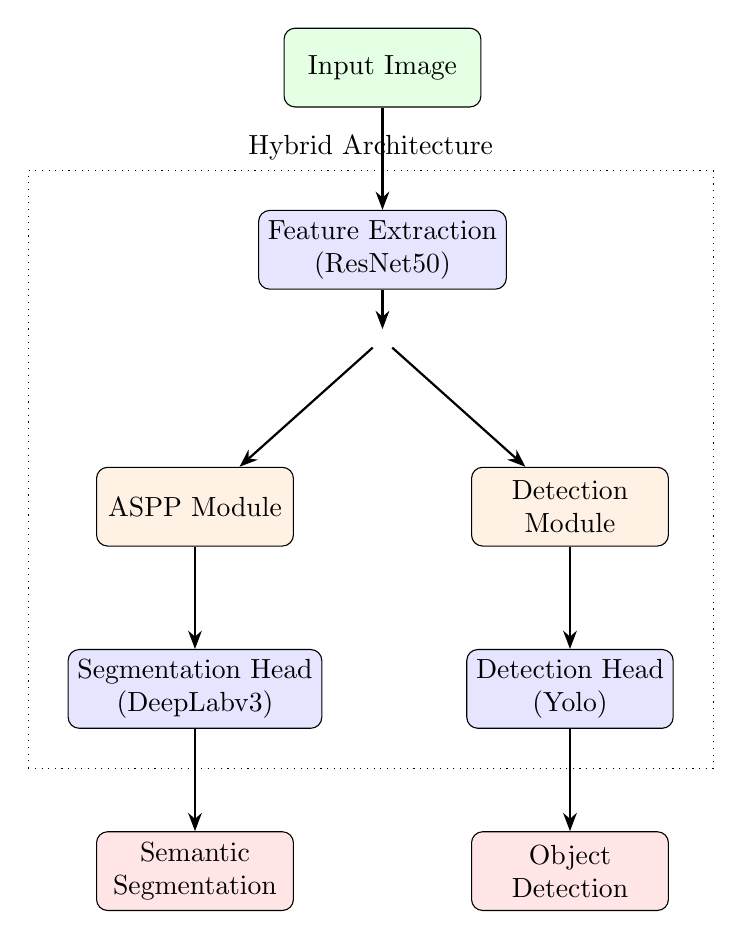
\begin{tikzpicture}[
        block/.style={draw, fill=blue!10, rounded corners, minimum width=2.5cm, minimum height=1cm, align=center},
        arrow/.style={-Stealth, thick},
        input/.style={draw, fill=green!10, rounded corners, minimum width=2.5cm, minimum height=1cm, align=center},
        output/.style={draw, fill=red!10, rounded corners, minimum width=2.5cm, minimum height=1cm, align=center},
        module/.style={draw, fill=orange!10, rounded corners, minimum width=2.5cm, minimum height=1cm, align=center},
        node distance=1.3cm
    ]
    
    % 输入节点
    \node[input] (input) {Input Image};
    
    % 特征提取节点
    \node[block, below=of input] (backbone) {Feature Extraction \\(ResNet50)};
    
    % 分支点
    \node[below=0.5cm of backbone] (branch) {};
    
    % DeepLabv3分支
    \node[module, below left=1.5cm and 1cm of branch] (aspp) {ASPP Module};
    \node[block, below=of aspp] (seghead) {Segmentation Head \\ (DeepLabv3)};
    \node[output, below=of seghead] (segout) {Semantic\\Segmentation};
    
    % YoloV3分支
    \node[module, below right=1.5cm and 1cm of branch] (detector) {Detection\\Module};
    \node[block, below=of detector] (dethead) {Detection Head\\ (Yolo)};
    \node[output, below=of dethead] (detout) {Object\\Detection};
    
    % 连接箭头
    \draw[arrow] (input) -- (backbone);
    \draw[arrow] (backbone) -- (branch);
    \draw[arrow] (branch) -- (aspp);
    \draw[arrow] (branch) -- (detector);
    \draw[arrow] (aspp) -- (seghead);
    \draw[arrow] (seghead) -- (segout);
    \draw[arrow] (detector) -- (dethead);
    \draw[arrow] (dethead) -- (detout);
    
    % 模型框架
    \node[draw, dotted, fit=(backbone)(aspp)(detector)(seghead)(dethead), inner sep=0.5cm, label=above:Hybrid Architecture] {};
    
    \end{tikzpicture}
    \caption{The proposed hybrid architecture combining YoloV3 for object detection and DeepLabv3 for semantic segmentation with a shared feature extraction backbone.}
    \label{fig:architecture}
\end{figure}

% 在这里Resnet50的细节架构见论文[1],我们不再赘述。在这主要介绍ASPP模块和Yolo的输出头。

For the detailed architecture of ResNet50, please refer to the paper [1], and we will not repeat it here. Here we mainly introduce the ASPP module and the output head of Yolo.

\begin{figure}[htbp]
    \centering
    \centerline{\includegraphics[width=0.5\textwidth]{fig/aspp.png}}
    \caption{ASPP Module Architecture}
    \label{fig:aspp}
\end{figure}

% ASPP模块是DeepLabv3的核心组件,它通过多尺度的空洞卷积来捕获不同尺度的上下文信息。在我们的模型中,我们使用了四个不同尺度的空洞卷积,分别是1、12、24、36,然后将它们拼接在一起,通过一个1x1的卷积层来融合这些信息。具体架构如下所示:

The ASPP module is the core component of DeepLabV3, which captures context information at different scales through multi-scale atrous convolutions. In our model, we use four different scales of atrous convolutions, namely 1, 12, 24, and 36, and then concatenate them together to fuse this information through a 1x1 convolutional layer. The specific architecture is as follows:

% YOLO 的输出头将会直接连接在ResNet50的输出上,他包含了全连接层和激活函数,最终输出的形状是(Sx,Sy,C+5B),其中Sx和Sy是图像块的维度,C是类别数,B是每个网格单元的边界框数。具体架构如下所示:

The output head of YOLO will be directly connected to the output of ResNet50, which includes fully connected layers and activation functions, and the final output shape is (Sx, Sy, C+5B), where Sx and Sy are the dimensions of the image block, C is the number of classes, and B is the number of bounding boxes per grid cell. The specific architecture is as follows:

\begin{figure}

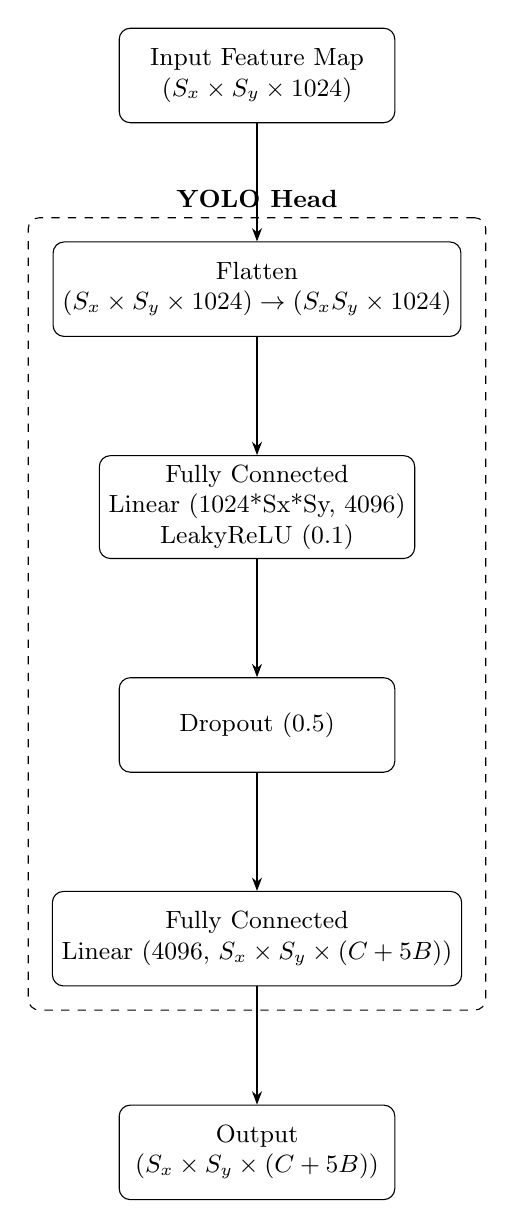
\begin{tikzpicture}[
    font=\small, 
    node distance=1.5cm, 
    >=Stealth, 
    block/.style={draw, rectangle, rounded corners, align=center, minimum width=3.5cm, minimum height=1.2cm},
    bigblock/.style={draw, dashed, rounded corners, inner sep=0.3cm}
]

% 输入特征图
\node[block] (input) {Input Feature Map\\\((S_x \times S_y \times 1024)\)};

% Flatten
\node[block, below=1.5cm of input] (flatten) {Flatten\\\((S_x \times S_y \times 1024) \to (S_x S_y \times 1024)\)};

% 全连接层1
\node[block, below=1.5cm of flatten] (fc1) {Fully Connected\\Linear (1024*Sx*Sy, 4096)\\LeakyReLU (0.1)};

% Dropout 层
\node[block, below=1.5cm of fc1] (dropout) {Dropout (0.5)};

% 全连接层2(最终输出)
\node[block, below=1.5cm of dropout] (fc2) {Fully Connected\\Linear (4096, \(S_x \times S_y \times (C + 5B)\))};

% 输出
\node[block, below=1.5cm of fc2] (output) {Output\\\((S_x \times S_y \times (C + 5B))\)};

% 连接箭头
\draw[->] (input.south) -- (flatten.north);
\draw[->] (flatten.south) -- (fc1.north);
\draw[->] (fc1.south) -- (dropout.north);
\draw[->] (dropout.south) -- (fc2.north);
\draw[->] (fc2.south) -- (output.north);

% 用虚线框标注 YOLO Head
\node[bigblock, fit=(flatten)(fc1)(dropout)(fc2), label=above:\textbf{YOLO Head}] (yolo_head) {};

\end{tikzpicture}

\caption{Yolo Output Head Architecture}
\label{fig:yolo}
\end{figure}

\subsection{Design Choices and Innovations}
% This subsection introduces the key decisions and specific optimizations made in the model design to adapt to the CamVid dataset.

% 在模型设计中,我们做出了一些关键决策和特定优化,以适应CamVid数据集。
% 对于语义分割来说,一个很重要的问题是如果按照典型的cnn模型进行连续的下采样和重复池化,不仅会导致最后特征图分辨率过低的问题,还会使得图中的大尺度和多尺度的物品被压缩进而丢失信息。在这我借用deepLabv3的思想,使用了ASPP模块来解决这个问题。ASPP模块通过多尺度的空洞卷积来捕获不同尺度的上下文信息,提高了模型的性能。此外我们还在ASPP模块的基础上进行了更新,使用空洞卷积来防止模型对大尺度物品丢失信息的情况。

% 对于物品检测,由于resnet作为特征提取头已经足够优秀,在这我们只需要将yolo的全连接层往下的层接入到resnet的输出上即可。这样可以避免因为过多的参数导致的过拟合问题。

In the model design, we made some key decisions and specific optimizations to adapt to the CamVid dataset.

For semantic segmentation, a critical issue is that if the typical CNN model is used for continuous downsampling and repeated pooling, it will not only lead to the problem of too low resolution of the final feature map but also compress large-scale and multi-scale objects in the image, resulting in information loss. Here, I borrowed the idea of DeepLabV3 and used the ASPP module to solve this problem. The ASPP module captures context information at different scales through multi-scale atrous convolutions, improving the performance of the model. In addition, we also updated the ASPP module to use atrous convolutions to prevent the model from losing information about large-scale objects.

For object detection, since ResNet as the feature extraction backbone is already excellent, we only need to connect the fully connected layers of Yolo to the output of ResNet. This can avoid the problem of overfitting caused by too many parameters.


\subsection{Training Strategy}
% This subsection introduces the training process, loss function selection, optimizer settings, and other details.

% 在训练过程中的损失函数上,我们使用了交叉熵损失函数来计算deeplab语义分割的损失,使用均方差来计算yolo目标检测的损失(和yolov1一样的损失函数计算方法)。在优化器上,我们使用了Adam优化器,并设置了初始学习率为 0.001,学习率衰减为0.1,一共训练100个epoch。同时设置早停机制,当验证集上的损失不再下降时,停止训练。记录训练数据和验证数据的损失,以便后续分析。

%同时为了提高训练速度,在合适的计算过程中我们开启了半精度计算(fp16)。

In the training process, we used the cross-entropy loss function to calculate the loss of Deeplab semantic segmentation and the mean square error to calculate the loss of Yolo object detection (the same loss calculation method as YoloV1). For the optimizer, we used the Adam optimizer, with an initial learning rate of 0.001, a learning rate decay of 0.1, and a total of 100 epochs. We also set up an early stopping mechanism to stop training when the loss on the validation set no longer decreases. We recorded the loss of the training data and validation data for subsequent analysis.

To improve training speed, we enabled mixed precision computing (fp16) in appropriate calculations.

\section{Experimental Setup}
% hyperparameters, etc.
\subsection{Experimental Environment}
This subsection describes the hardware and software environment used for the experiments.

\subsection{Hyperparameter Settings}
This subsection lists in detail the hyperparameters used in the training process, such as learning rate, batch size, number of epochs, etc., and explains the reasons for these choices.

\subsection{Evaluation Metrics}
This subsection explains the metrics used to evaluate model performance, such as mAP, IoU, etc., and the calculation methods for these metrics.

\section{Results}
% mAP/IoU scores, class-wise analysis, qualitative results
\subsection{Overall Performance}
This subsection presents the overall performance of the model on the test set, including average precision and IoU scores.

\subsection{Class Analysis}
This subsection analyzes the performance differences across classes, identifying which classes perform well and which perform poorly, and discussing possible reasons.

\subsection{Qualitative Results}
This subsection presents some intuitive visual results, comparing model predictions with ground truth annotations.

\section{Class Imbalance}
% Techniques tested, impact on performance, comparison
\subsection{Class Imbalance Handling Techniques}
This subsection introduces various techniques tested to address the class imbalance issues in the dataset, such as resampling, weighted loss functions, etc.

\subsection{Impact on Performance}
This subsection analyzes the impact of various class imbalance handling techniques on overall model performance and performance across different classes.

\subsection{Technique Comparison}
This subsection compares the advantages and disadvantages of different techniques and proposes the most suitable solution for this task.

\section{Discussion}
% discuss results and limitations
\subsection{Result Analysis}
This subsection provides an in-depth discussion of the experimental results, analyzing the strengths and weaknesses of the model.

\subsection{Limitations}
This subsection honestly points out the limitations of the research, such as dataset constraints, computational resource limitations, etc.

\subsection{Potential Applications}
This subsection explores the potential uses of the model in practical application scenarios, especially in the field of robotics.

\section{Conclusion}
% Lessons learned, future work
This section summarizes the main findings and contributions of the research. It reflects on the lessons learned throughout the research process and proposes possible future research directions and improvements.

% Keep the original references format and acknowledgment section
\section*{Acknowledgment}
Thanks to [relevant personnel/institutions] for their support of this research.

\begin{thebibliography}{00}
\bibitem{b1} [YoloV3 related citation]
\bibitem{b2} [Deeplabv3 related citation]
\bibitem{b3} [CamVid dataset related citation]
\bibitem{b4} [Class imbalance problem related citation]
\bibitem{b5} [Semantic segmentation evaluation method related citation]
\end{thebibliography}

\end{document}